\newpage
  \begin{center}
  \section{ }%Как посчитать щели
  \label{sec:_}
  \end{center}
Получить формулу

$$ f_d^2 = \frac{f_S^2}{b_S}+\frac{f_M^2}{b_M}+\left( \frac{\Delta \lambda}{\lambda} (\tan(\theta_B^S) - \tan(\theta_B^M)) \right)^2  $$


\begin{figure}[H]
  \centering
  \subfloat[f = 3, $\theta_B^M - \theta_B^S = 0$]{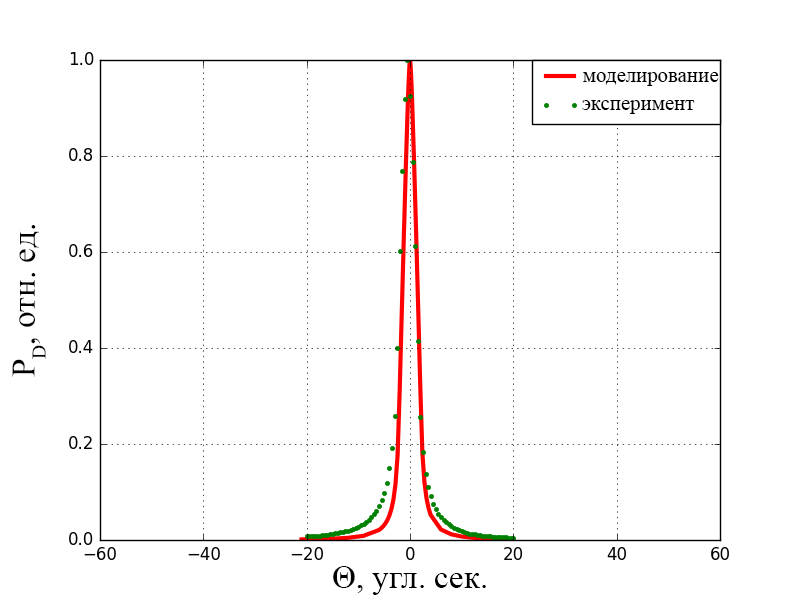
\includegraphics[width=0.3\textwidth]{images/220_440_660/220.png}}
  \hfill
  \subfloat[f = 18, $\theta_B^M - \theta_B^S = 11$]{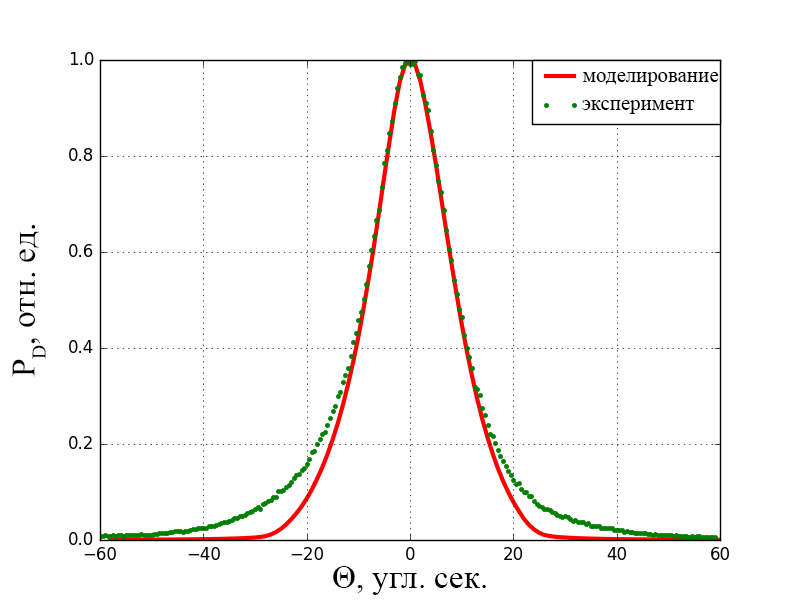
\includegraphics[width=0.3\textwidth]{images/220_440_660/440.png}}
  \hfill
  \subfloat[f = 39, $\theta_B^M - \theta_B^S = 23$]{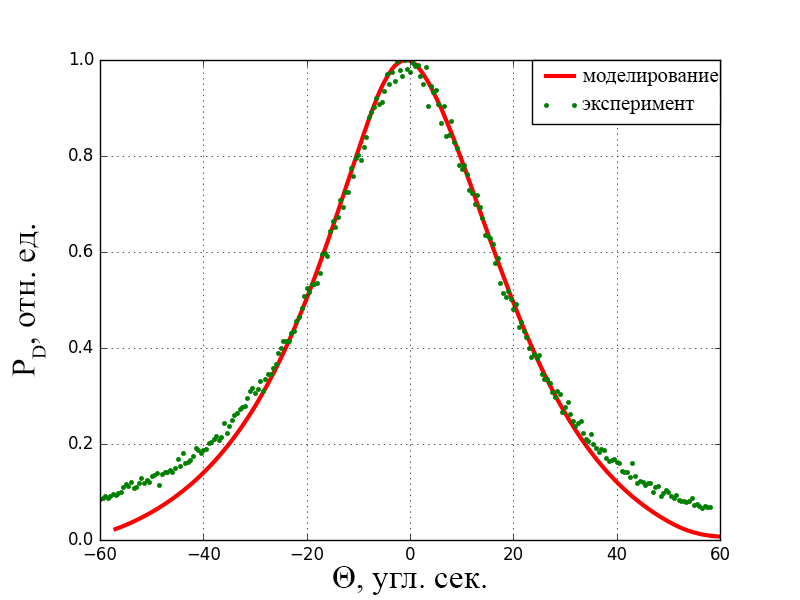
\includegraphics[width=0.3\textwidth]{images/220_440_660/660.png}}
  \caption{Дисперсия}
  \label{ris:}
\end{figure}
